\documentclass{standalone}
\usepackage{tikz}
\usepackage{ctex,siunitx,ninecolors}
\setCJKmainfont{Noto Serif CJK SC}
\usepackage{tkz-euclide}
\usepackage{amsmath}
\usetikzlibrary{patterns, calc}
\usetikzlibrary {decorations.pathmorphing, decorations.pathreplacing, decorations.shapes}
\begin{document}
\small
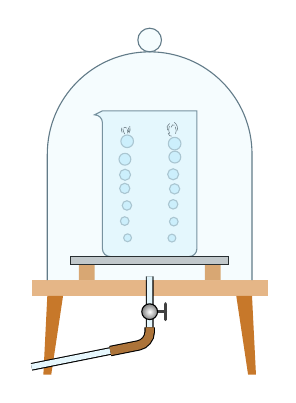
\begin{tikzpicture}[>=latex,scale=1.0]
  % \useasboundingbox(-1.4,-1.4)rectangle(1.4,1.4);
  \foreach \y[count =\i] in {1.45,1.65,...,2.65}
  {
    \fill[cyan!20!white,draw=cyan!20!gray](-0.3+0.02*rand,\y+0.02*rand)circle(0.045+0.005*\i);
    \fill[cyan!20!white,draw=cyan!20!gray](0.3+0.02*rand,\y+0.02*rand)circle(0.045+0.005*\i);
  }
  \draw[very thin] (-0.349,2.776)..controls(-0.365,2.794)and(-0.359,2.817)..(-0.353,2.838)
  (-0.318,2.755)..controls(-0.318,2.789)and(-0.349,2.794)..(-0.340,2.821)
  (-0.331,2.831)..controls(-0.319,2.848)and(-0.309,2.845)..(-0.289,2.831)
  (-0.281,2.764)..controls(-0.276,2.780)and(-0.275,2.800)..(-0.285,2.814)
  (-0.267,2.783)..controls(-0.262,2.807)and(-0.263,2.823)..(-0.272,2.836)
  (-0.253,2.856)..controls(-0.241,2.821)and(-0.249,2.784)..(-0.263,2.767)
  (0.227,2.806)..controls(0.209,2.843)and(0.224,2.865)..(0.253,2.890)
(0.255,2.762)..controls(0.235,2.804)and(0.241,2.823)..(0.250,2.857)
(0.235,2.769)..controls(0.241,2.736)and(0.261,2.726)..(0.278,2.730)
(0.273,2.841)..controls(0.277,2.875)and(0.295,2.879)..(0.318,2.869)
(0.324,2.849)..controls(0.343,2.817)and(0.340,2.785)..(0.329,2.759)
(0.313,2.906)..controls(0.348,2.875)and(0.359,2.842)..(0.357,2.802);
  \draw[cyan!30!darkgray,fill=cyan!20,fill opacity=0.4](-0.7,3.0)arc(90:0:0.1)--(-0.6,1.3)arc(-180:-90:0.1)--(0.5,1.2)arc(-90:0:0.1)--(0.6,3.05)--(-0.6,3.05)--cycle;
  \fill[brown7](-0.7,1.1)rectangle(-0.9,0.9)(0.7,1.1)rectangle(0.9,0.9);
  \draw[fill=lightgray](-1.0,1.1)rectangle(1.0,1.2);
  \fill[brown8](-1.5,0.9)rectangle(1.5,0.7);
  \fill[brown6](1.3,0.7)--(1.35,-0.3)--(1.25,-0.3)--(1.1,0.7)(-1.3,0.7)--(-1.35,-0.3)--(-1.25,-0.3)--(-1.1,0.7);
  \draw[double=cyan!10!white,double distance=2pt,rounded corners](0,0.95)--(0,0.1)--(-1.5,-0.2);
  \draw[double=brown!90!black,double distance=3pt,rounded corners](0,0.3)--(0,0.1)--(-0.5,0);
  \draw[darkgray,very thick,line cap=round](0,0.5)--++(0.2,0)(0.2,0.4)--(0.2,0.6);
  \draw[inner color=white,outer color=gray](0,0.5)circle(0.1);
  \draw[cyan!30!darkgray,fill=cyan!20,fill opacity=0.2](-1.3,0.9)--(-1.3,2.5)arc(180:0:1.3)--(1.3,0.9);
  \draw[cyan!30!darkgray,fill=cyan!20,fill opacity=0.2](0,3.95)circle(0.15);
\end{tikzpicture}
\end{document}